\documentclass[25pt]{sciposter}

\usepackage[T1]{fontenc}
\usepackage[utf8]{inputenc}

\usepackage{amsthm}

\usepackage[dvipsnames,usenames,svgnames,table]{xcolor} 
\usepackage{lipsum}
\usepackage{epsfig}
\usepackage{amsmath}
\usepackage{amssymb}

\usepackage[german]{babel}
\usepackage{geometry}
\usepackage{multicol}
\usepackage{graphicx}
\usepackage{tikz}
\usepackage{wrapfig}
\usepackage{gensymb}
\usepackage{tocloft}
\usepackage{empheq}

\usepackage{pgfplots}
\pgfplotsset{width=11cm,compat=1.9}


% for nice tableas
\usepackage{booktabs}

\graphicspath{ {img/} }

\geometry{
 landscape,
 a1paper,
 left=5mm,
 right=50mm,
 top=5mm,
 bottom=50mm,
 }
\usepackage{array}   % for \newcolumntype macro
\newcolumntype{L}{>{$}m{5.5cm}<{$}} % math-mode version of "l" column type

%BEGIN LISTINGDEF


\newtheorem*{lem}{Lemma}


\newcommand*\widefbox[1]{\fbox{\hspace{2em}#1\hspace{2em}}}
\newcommand{\limm}{\lim\limits_{n \to \infty}}
\newcommand{\limx}[1]{\lim\limits_{x \to #1}}
\newlength\dlf  % Define a new measure, dlf
\newcommand\alignedbox[2]{
% Argument #1 = before & if there were no box (lhs)
% Argument #2 = after & if there were no box (rhs)
&  % Alignment sign of the line
{
\settowidth\dlf{$\displaystyle #1$}
    % The width of \dlf is the width of the lhs, with a displaystyle font
\addtolength\dlf{\fboxsep+\fboxrule}
    % Add to it the distance to the box, and the width of the line of the box
\hspace{-\dlf}
    % Move everything dlf units to the left, so that & #1 #2 is aligned under #1 & #2
\boxed{#1 #2}
    % Put a box around lhs and rhs
}
}
\usepackage{graphicx,url}

%BEGIN TITLE
\title{\huge{Informationstheorie}}

\author{\large{David Zollikofer}}
%END TITLE


%\usepackage{eulervm}
\usepackage{mathpazo}
% begin custom commands
\newcommand{\Q}{\mathbb{Q}}
\newcommand{\R}{\mathbb{R}}
\newcommand{\N}{\mathbb{N}}
\newcommand{\F}{\mathcal{F}}
\newcommand{\X}{\mathcal{X}}
\newcommand{\W}{\mathcal{W}}
\newcommand{\Nor}{\mathcal{N}}
\newcommand{\U}{\mathcal{U}}
\newcommand{\Var}{\operatorname{Var}}
\newcommand{\E}{\operatorname{E}}
%\newcommand{\exp}{\operatorname{exp}}
\newcommand{\C}{\mathcal{C}}
\newcommand{\mc}{\mathcal}

% some shortcuts
\newcommand{\ds}{\displaystyle}
\newcommand{\arr}{\rightarrow}
\newcommand{\nop}[1]{}
\renewcommand{\hat}{\widehat}

% stuff for integrals
\newcommand{\intl}{\int\limits}
\newcommand{\rmd}{\mathrm{d}}


\newcommand{\norm}[1]{\left\lVert#1\right\rVert}
\usepackage[framemethod=latex]{mdframed}
\newenvironment{defn}[1]{\begin{mdframed}[backgroundcolor=blue!10,innertopmargin=15pt, nobreak=true,innerbottommargin=15pt]
		\textbf{#1 }
	}
	{ 
	\end{mdframed}
}

\newenvironment{important}{\begin{mdframed}[backgroundcolor=red!50,innertopmargin=15pt, innerbottommargin=15pt, nobreak=true]
		\Large
	}
	{ 
	\end{mdframed}
}

\newenvironment{lemma}{\begin{mdframed}[backgroundcolor=gray!50,innertopmargin=15pt, innerbottommargin=15pt, nobreak=true]
		\Large
	}
	{ 
	\end{mdframed}
}

\newenvironment{thm}[1]{\begin{mdframed}[nobreak=true,backgroundcolor=Emerald!10,innertopmargin=15pt, innerbottommargin=15pt]
		\textbf{#1 }
	}
	{ 
	\end{mdframed}
}



\newenvironment{trick}[1]{\begin{mdframed}[backgroundcolor=PineGreen!50,innertopmargin=15pt, innerbottommargin=15pt, nobreak=true]
			\textbf{#1 }
	}
	{ 
	\end{mdframed}
}


\usepackage{todonotes}
\newcommand{\TODO}[1]{\todo[inline]{\Large TODO:  #1}}





\DeclarePairedDelimiter\abs{\left|}{\right|}%



\setlength\abovedisplayskip{0pt}

\renewcommand{\familydefault}{\rmdefault}

% end custom commands

\begin{document}





\maketitle



\begin{multicols}{3}



\textit{Diese Zusammenfassung fasst die wichtigsten Definitionen und Theoreme der Informationstheorie Vorlesung gehalten von Dr. Luis Haug im Frühling 2020 zusammen. Alle Beweise finden sich entweder im Skript oder den Übungen und wurden hier weggelassen.}


\section{Entropie}


Die Entropie misst die Unsicherheit über den Wert eine Zufallsvariable $X$ bevor wir ihn erfahren.

\begin{defn}{Entropie einer Zufallsvariable}
Sei $X:\Omega \to \mathcal{X}$ mit Verteilung $P_X$ so dass $H(X) = H(P_X)$ so gilt

\begin{align*}
	H(X) := - \sum_x P_X(x) \log P_X(x)
\end{align*}
\end{defn}

\begin{defn}{Gemeinsame Entopie}
Die gemeinsame Entropie zweier Zufallsvariablen $(X,Y)$ mit $X:\Omega \to \mathcal{X}$ sowie $Y\to \mathcal{Y}$ mit gemeinsamer Verteilung $P_{X,Y}$ ist

\begin{align*}
	H(X,Y) = - \sum_{x,y} P_{X,Y} (x,y) \log P_{X,Y} (x,y)
\end{align*}
\end{defn}

\begin{defn}{Entropie bedingter Verteilung}
	Für $y\in Y(\Omega)$ mit $P_Y(y) > 0$ haben wir die auf $Y=y$ bedingte Verteilung $P_{X|Y=y}$ mit 
	\begin{align*}
		P_{X|Y=y} &= P(X=x | Y = y) = \frac{P_{X,Y}(x,y)}{P_Y(y)}
	\end{align*}
	
	für welche gilt
	
	\begin{align*}
	H(X|Y=y) = - \sum_{x} P_{X|Y=y} (x) \log P_{X|Y=y} (x)
	\end{align*}
	was die Unsicherheit über $X$ misst wenn $Y=y$ bekannt ist.
\end{defn}

\begin{defn}{Bedingte Entropie}
	Gegeben Zufallsvariablen $X,Y$ so definieren wir die bedingte Entropie von $X$ gegeben $Y$ als
	
	\begin{align*}
		H(X|Y) = \sum_y P_Y(y) H(X|Y=y)
	\end{align*}
	
	wobei $H(X|Y)$ der Erwartungswert von $H(X|Y=y)$ bezüglich aller möglichen $y$ ist.
\end{defn}

\begin{thm}{Kettenregel}
	Für jedes Paar an Zufallsvariablen $X,Y$ gilt
	\begin{align*}
		H(X|Y) + H(Y) = H(X,Y) = H(Y|X) + H(X)
	\end{align*}
\end{thm}

\begin{thm}{Erweiterte Kettenregel}
	Es gilt durch mehrfaches anwenden der Kettenregel, dass
	
	\begin{align*}
		H(X_1,\ldots,X_n) &= H(X_1) + \sum_{i=2}^{n} H(X_i | X_1,\ldots X_{i-1})
	\end{align*}
	
	Ausgeschrieben wäre dies:
	$$H(X,Y,Z) = H(X) + H(Y|X) + H(Z|X,Y)$$
\end{thm}


\begin{defn}{Wechselseitige Information}
	Wir definieren 
	
	\begin{align*}
		I(X;Y) = H(X) - H(X|Y)
	\end{align*}
	
	als die Reduktion der Unsicherheit über $X$ durch Bekanntwerden von $Y$.
	
	Aufgrund der Kettenregel gilt
	
	\begin{align*}
		I(X;Y) &= H(X) + H(Y) - H(X,Y) = I(Y;X)
	\end{align*}
	
\end{defn}


	\begin{thm}{Satz zur wechselseitigen Information}
	Für alle $X,Y$ gilt $I(X;Y)\geq 0$ mit Gleichheit wenn $X,Y$ unabhängig sind.	
\end{thm}


\begin{defn}{Kullback-Leibler-Divergenz}
	Die Kullback-Leibler-Divergenz zwischen zwei Zufallsvariablen $P,Q$ ist definiert durch
	
	\begin{align*}
		D_{KL} (P||Q) = -\sum_{\omega}P(\omega) \log\left( \frac{Q(\omega)}{P(\omega)} \right) = \E \left[\log\frac{P}{Q}\right]
	\end{align*}
\end{defn}

\begin{thm}{Gibbs Ungleichung}
	Es gilt $D_{KL}(P||Q)\geq 0 $ mit Gleichheit genau dann wenn $P=Q$.
\end{thm}


\begin{figure}
	\centering
	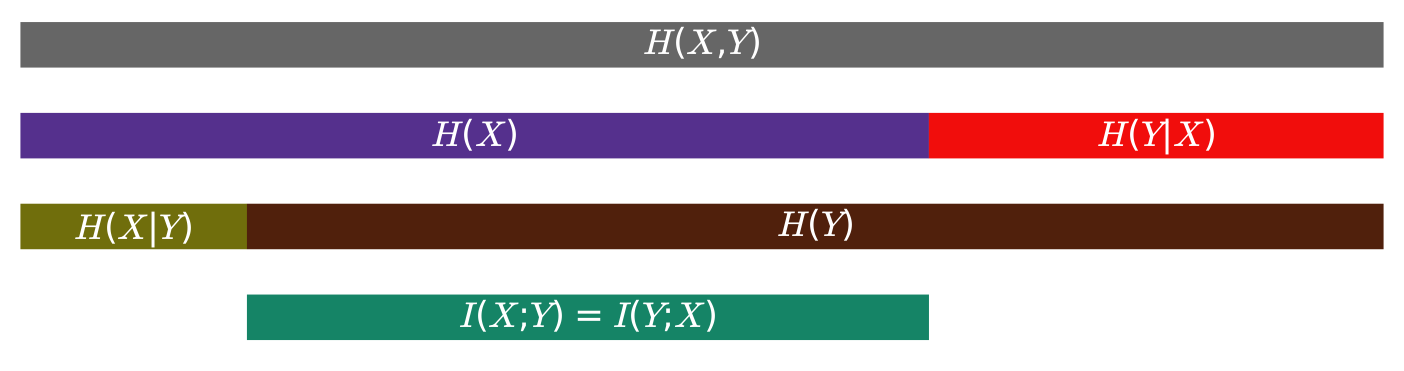
\includegraphics[width=1\linewidth]{overviewChpt1}
	\caption{Übersicht der relevanten Grössen}
	\label{fig:overviewchpt1}
\end{figure}
\begin{defn}{Bedingte Gegenseitige Information}
	Die bedingte Gegenseitige Information, die $X$ über $Y$ gibt, gegeben $Z$ ist 
	
	\begin{align*}
	I(X;Y|Z) &= H(XZ) + H(YZ)- H(XYZ) - H(Z)
	\end{align*}
	
	Am besten erklärt man sich dies Intuitiv durch die Regel $I(X;Y) = H(X) + H(Y) - H(XY)$ wobei man immer auf $Z$ bedingt und dann auflöst.
	
\end{defn}

\begin{figure}
	\centering
	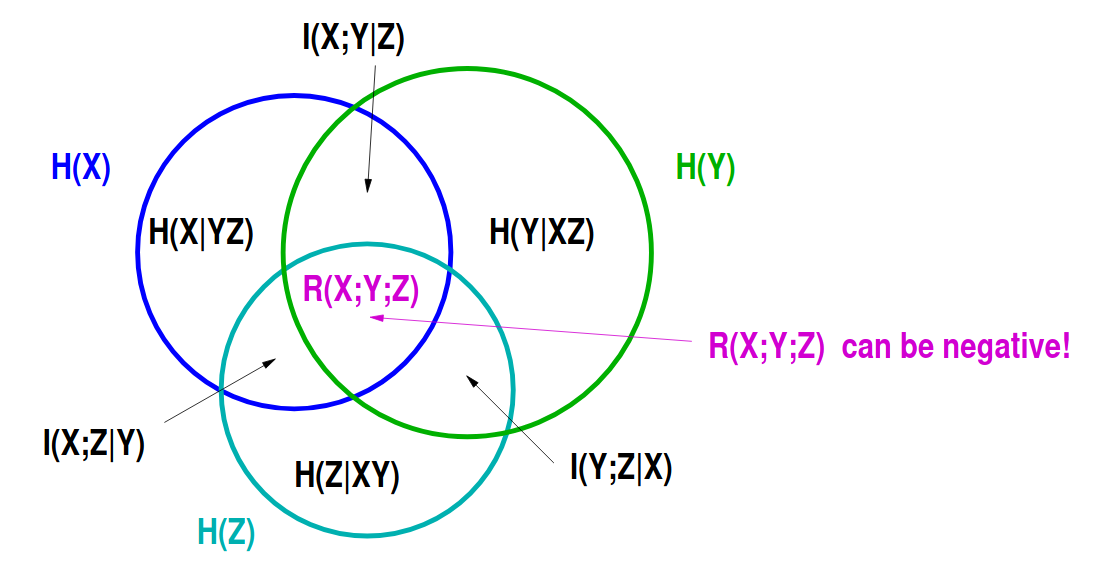
\includegraphics[width=0.8\linewidth]{overviewChpt2}
	\caption{Übersicht (Quelle: Information und Kommunikation Prof. U. Maurer)}
	\label{fig:overviewchpt2}
\end{figure}


\section{Quellcodierung}


\begin{defn}{Quellcode} Ein Quellcode über einem Alphabet $\mathcal{D}$ für eine Menge $\mathcal{X}$ ist eine Abbildung $C:\mathcal{X} \to \mathcal{D}^*$. Dabei ist $C(x)$ ein Codewort für $x\in \mathcal{X}$. Die Länge von $C(x)$ wird als $l_C(x)$ bezeichnet.
\end{defn}

\textbf{Ziel:} Wir möchte gerne die erwartete Länge eines Codes $C$

\begin{equation*}
L_C = \E[l_C] = \sum_{x\in X(\Omega)} P_X(x) l_C(x)
\end{equation*}
so klein wie möglich haben.




\begin{defn}{Eigenschaften von Codes}
	\begin{itemize}
		\item Ein Code $C$ heisst \textbf{nicht degeneriert}, falls $$x_i \neq x_j \implies C(x_i) \neq C(x_j) \quad \forall i\neq j$$
		\item Wir nennen $C$ \textbf{präfixfrei}, falls kein Codewort $C(x)$ ein Präfix eines anderen Codewortes ist.
	\end{itemize}
\end{defn}

Wir erweitern nun den Code $C$ zu einem Code $C^*$ für welchen $C^*(x_1 \ldots x_n) \mapsto C(x_1)\ldots C(x_n)$ gilt. Wenn $C^*$ nicht degeneriert ist, so nennen wir $C^*$ \textbf{eindeutig dekodierbar}.

\begin{thm}{Kraft Ungleichung}
\begin{itemize}
	\item Für jeden präfixfreien Code $C:{X}(\Omega)\to \{0,1\}^*$ gilt 
	
	$$\sum_{x \in X(\Omega)} 2^{-l_C(x)} \leq 1$$
	
	\item Falls eine Funktion $l:X(\Omega)\to\N$ die Ungleichung
	
	$$\sum_{x\in X} 2^{-l(x)} \leq 1$$
	
	erfüllt, so existiert ein präfixfreier Code $C:X(\Omega) \to \{0,1\}^*$, so dass $l_C(x) = l(x)$.
\end{itemize}
\end{thm}

\begin{defn}{Optimaler Code}
	Wir nennen einen Code ${C'}:{X}(\Omega^) \to \{0,1\}^*$ optimal, falls für jeden anderen Code $C$ für $\mathcal{X}$ gilt $L_{C'} \leq L_C$. 
\end{defn}



\begin{thm}{Minimale Länge eines präfixfreien Codes}
Die erwartete Länge jedes präfixfreien Codes $C: X(\Omega) \to \{0,1\}^*$ erfüllt $L_C \geq H(X)$. Um $L_C = H(X)$ zu erreichen muss $p_i = 2^{-l_i}$ für alle $i$ mit $l_i \in \N$ sein.
\end{thm}

\begin{thm}{Existenz fast optimaler Codes}
		Jeder optimale präfixfreie Code $C':X(\Omega) \to \{0,1\}^*$ erfüllt 
		
		\begin{align*}
			H(X) \leq L_{C'} < H(X) + 1
		\end{align*}
		
		Diese Schranke erreichen wir indem wir indem wir $l_i := \lceil -\log p_i \rceil$ fordern.
		
		Wenn wir jeweils Blöcke der Länge $N$ Codieren so gilt 
		
		\begin{align*}
			H(X) \leq \frac{1}{N} L_{C_N} < H(X) + \frac{1}{N}
 		\end{align*}
womit insbesondere $\lim_{N\to \infty} L_{C_N} = H(X)$.

\end{thm}

 
\begin{thm}{Codes bezüglich falscher Verteilung}
		Wenn wir einen optimalen Code $C_q$ mit $l_{C_q}(x_i) = \lceil-\log q(x_i) \rceil$ verwenden um eine Eingabe mit der Verteilung $p$ zu Enkodieren so gilt
	
	\begin{align*}
		H(X) + D_{KL}(p||q) \leq \E_p[l_{C_q}] < H(X) + D_{KL}(p||q)  + 1
	\end{align*} 
	Wir bezahlen demnach also eine Strafe von $D_{KL}(p||q)$.
	
\end{thm}


\paragraph{Konstruktion von Huffman-Codes}
	Für eine Verteilung von $X$ gegeben durch $\vec{p} = (p_1,\ldots,p_n)$ konstruieren wir einen Huffman-Code rekursiv:
	\begin{itemize}
		\item Wähle die zwei kleinsten Wahrscheinlichkeiten $p_i$ und $p_j$.
		\item Wähle beide als Blätter und baue einen Baum aus drei Knoten wobei der Elternknoten die Wahrscheinlichkeit $p' = p_i + p_j$ hat. Gebe dem einen Kind $p_i$ den Präfix $1$, dem anderen $p_j$ den Präfix $1$.
		\item Entferne $p_i,p_j$ aus $\vec{p}$ und füge $p'$ zu $\vec{p}$ als neues Ereignis hinzu.
		\item Iteriere bis $\vec{p}$ nur noch ein Element hat mit $p_i = 1$, der Baum der zu dieser Wahrscheinlichkeit gehört ist der Huffman-Baum
	\end{itemize}


\begin{thm}{Optimalität von Huffman-Codes}
Sei ${C_H}$ ein Huffman-Code für eine Zufallsvariable $X$ und sei $C^*$ ein optimaler präfixfreier Code für $X$, so ist $C_H$ ebenfalls ein optimaler Code für $X$ da gilt:
\begin{align*}
	L_{C_H} &= L_{C^*}
\end{align*}
\end{thm}

\begin{thm}{McMillan Ungleichung}
Jeder eindeutig dekodierbare Code $C:\mathcal{X}\to \{0,1\}^*$ erfüllt die Kraftungleichung
\begin{align*}
	\sum_{x\in\mathcal{X}} 2^{-l_C (x)} \leq 1
\end{align*}
\end{thm}

Daher folgt, dass es eigentlich reicht präfixfreie Codes anzuschauen, da allgemeine dekodierbare Codes die gleichen Eigenschaften haben.

%\vfill\null
%\columnbreak

\begin{defn}{Typische Folgen}
	Wir typische Ereignisse $\vec{x}$ auf $X^N$ Ereignisse die bei Erfolgswahrscheinlichkeit Bernoulli $p$ etwas mit Wahrscheinlichkeit $p^{pN} (1-p)^{(1-p)N}$ vorkommen.
	
	Für ein solche solches $\vec{x}$ gilt dann
	\begin{align*}
		-\frac{1}{N} \log P(\vec{x}) = - \frac{1}{N} \log \left( p^{pN} (1-p)^{(1-p)N}\right) = H(p,1-p)
	\end{align*} 
\end{defn}


\begin{defn}{Typische Menge}
	
	Für $\epsilon, N$ gegeben ist die typische Menge
	
	\begin{align*}
		T_{N,\epsilon} &= \bigg\{ \vec{x} \in \mathcal{X}^N |  \left| -\frac{1}{N}\log P(\vec{x}) - H(X) \right|  \leq \epsilon \bigg \}\\
		&= \bigg\{ \vec{x} \in \mathcal{X}^N | 2^{-N(H(X)+\epsilon)} < P(\vec{x}) < 2^{-N(H(X)-\epsilon)} \bigg \}
	\end{align*}
\end{defn}


\begin{thm}{Asymptotische Gleichverteilungseigenschaft}
	Falls die Zufallsvariablen $X,X_1,\ldots,x_n:\Omega\to \mathcal{X}$ i.i.d. sind, so gilt
	\begin{align*}
P\left( \left| -\frac{1}{N}\log P(X_1,\ldots,X_n) - H(X) \right|  > \epsilon \right) \to 0  \text{ für } N \to \infty
	\end{align*}
	
	Als Korollare folgen
	\begin{enumerate}
		\item $P(T_{N,\epsilon}) \to 1$ für $N \to \infty$
		\item $|T_{N,\epsilon}| < 2^{N(H(X) + \epsilon)}$
		\item $|T_{N,\epsilon}| > (1-\delta)2^{N(H(X)) - \epsilon}$ für jedes $\delta \in (0,1)$ und $N \gg 1$.
	\end{enumerate}
\end{thm}


\begin{defn}{Datenkompression via AEP}
Wir codieren mit Blockcode $C:\mathcal{X}^N \to \{0,1\}^*$ mit 
\begin{align*}
	C(x) \mapsto \begin{cases}
	"1" + \{0,1\}^{\lceil N(H(X) + \epsilon) \rceil} \ \text{ für } x \in T_{N,\epsilon}\\
	"0" + \{0,1\}^{N\log |\mathcal{X}|}
	\end{cases}
\end{align*}
für diesen Code gilt $L_C \leq N(H(X) + \epsilon')$ was pro Symbol eine Länge von $H(X)$ gibt bei grossem $N$.
\end{defn}



\begin{thm}{Shannons Quellcodierungstheorem} Sei $H_\delta(X)$ die kleinste Anzahl an Bits um eine Menge $S_\delta$ mit $P(S_\delta)\geq 1-\delta$ zu beschreiben, dann gilt für alle $\epsilon > 0$ und $\delta\in (0,1)$ dass es ein $N_0 \in \N$ gibt, so dass für alle $N \geq N_0$
	
	\begin{align*}
\left|\frac{1}{N} H_{\delta} (X^N) - H(X) \right| < \epsilon
	\end{align*}
gilt. Dies hat zwei Konsequenzen:

\begin{itemize}
	\item Wir brauchen nur $H(X)$ Bits pro Symbol
	\item Auch wenn wir eine hohe Fehlerwahrscheinlichkeit in Kauf nehmen ($\delta$ gross), so benötigen wir immer noch $H(X)$ Bits für die Elemente in $S_\delta$.
\end{itemize}

\end{thm}


\paragraph{Arithmetische Codes}
Wir fügen unserem Alphabet $\{s_1,\ldots ,s_{M-1}\}$ das ein end-of-file symbol $s_M = \square$ hinzu.

Angenommen wir haben ein probabilistisches Modell $P(X_N = s_i | X_1, \ldots X_{N-1})$ 

Wir starten mit $[0,1)$ und bauen rekursive Intervalle $I_m$ mit der Länge von $I_m = P(X_1 = s_m)$. Nun unterteilen wir $I_m$ wieder in $I_{m,m'}$ mit der Länge von $I_{m,m'}$ proportional zu $P(X_2 = s_{m'} | X_1 = s_m)$. (Dies wiederholen wir nun rekursiv).

Wir kriegen somit Binärintervalle der Form 
\begin{align} \label{binString}
	\left[ \sum_{i=1}^{N} b_i 2^{-i},2^{-N} \sum_{i=1}^{N} b_i 2^{-i} \right), \quad b_i \in \{0,1\}
\end{align}
Dabei nutzen wir nun den String der Binärzahl $ \sum_{i=1}^{N} b_i 2^{-i}$ als Code für ein Wort das in dieses Intervall fällt.


Dabei sind:

\begin{itemize}
	\item $B_i$ ein Intervall das durch einen Binärstring $b_i$ beschrieben wird nach (\ref{binString})
	\item $I_n$ ein Intervall nach rekursiver Definition durch Wahrscheinlichkeiten.
\end{itemize}


Dabei gilt:


\begin{lem}
	Seien $\vec{x}, \vec{x}' \in \{s_1,\ldots,s_m\}^*$. Es gilt $I_{\vec{x}'} \subseteq I_{\vec{x}}$ gdw. $\vec{x}$ ein Präfix von $\vec{x}'$ ist.
\end{lem}

\begin{lem}
	Seien $\vec{x}, \vec{x}' \in \{s_1,\ldots,s_m\}^*$ und $\vec{b}, \vec{b}' \in \{0,1\}^*$ mit
	\begin{align*}
		I_{\vec{x}'} &\subset B_{\vec{b}'} & B_{\vec{b}} &\subset I_{\vec{x}}
	\end{align*}
	Falls $\vec{x}'$ ein Präfix von $\vec{x}$ ist, dann ist $\vec{b}'$ ein Präfix von $\vec{b}$.
\end{lem}
Dies erlaubt uns schon während des Empfangs des Codeworts mit dekodieren zu beginnen.


\paragraph{Lempel-Ziv-Codes}
	\textit{Enkodieren:}	Wir möchten kodieren und kennen die Auftretwahrscheinlichkeiten noch nicht. Dafür nehmen wir einen Eingabestring und bauen nach jedem Substring den wir noch nicht gesehen haben $|$ ein.
	
	\texttt{|1|0|11|01|010|00|10}
	
	Daraus bauen wir das Wörterbuch
	
{
	\begin{tabular}{|c|c|c|c|c|c|c|c|c|}
	\hline
	Wort & $\lambda$ & \texttt{1} & \texttt{0}  & \texttt{11} & \texttt{01} & \texttt{010} & \texttt{00} & \texttt{10} \\
	\hline
	$s(n)$& 0 & 1 & 2 & 3 & 4 & 5 & 6 & 7 \\
	\hline
	 $s_{bin}(n)$ & 000 & 001 & 010 & 011 & 100 & 101 & 110 & 111 \\
	\hline
	(ptr,bit) & & (,1) & (0,0) & (01,1) & (10,1) & (100,0) & (010,0) & (001,0)\\ 
	\hline
\end{tabular}}
Dabei habe wir den Pointer jeweils $\lceil \log_2 s(n) \rceil$ lang gemacht, sowie den ersten Pointer weggelassen.

Das Resultat wäre dann \texttt{100011101100001000010}


\textit{Dekodieren:} Wir nehmen den String und unterteilen ihn in jeweils $2^{k-2}$ Phrasen der Länge $k$, wobei wir das erste Bit separat betrachten.

Dies gibt \texttt{1|00|011|101|1000|0100|0010}
Hierbei ist das letzte Bit im Block das neue Bit und alle vorhergehenden sind Pointer.


\paragraph{Zusammenfassend}

Alle kennengelernten Kodierungsverfahren sind optimal!


\section{Kanalkodierung}


\begin{defn}{Disreter gedächtnisloser Kanal}
	Ein diskreter gedächtnisloser Kanal besteht aus einem Eingabealphabet $\mathcal{X}$, einem Ausgabealphabet $\mathcal{Y}$ und einer Familie $(P(\cdot|x))_{x\in \mathcal{X}}$ von Verteilungen auf $\mathcal{Y}$
	
	Dabei heisst Gedächtnislos, dass das soeben Empfangene Bit nicht von früheren abhängt, wobei $P(x|y)$ für die Wahrscheinlichkeit, dass $x$ empfangen wird, wenn $y$ gesendet wurde.
\end{defn}

\begin{defn}{Kanalkapazität}
	Wenn $H(X)$ an Entropie gesendet wird und wir $H(Y)$ empfangen, so wollen wir die Unsicherheit $H(X|Y)$ möglichst klein halten. Da $H(X) - H(X|Y) = I(X;Y)$ definieren wir die Kapazität $C$ eines Kanals
	
	\begin{align*}
		C = \max_{P_X}I(X;Y)
	\end{align*}
\end{defn}


\subsection*{Beispiele von Kanälen}

\paragraph{Binärer symmetrischer Kanal}
Der Kanal hat nur \texttt{0} und \texttt{1} als Zustand wobei die Chance dass ein Bit falsch übetragen wird symmetrisch bei $p$ liegt.

Es gilt dabei $I(X;Y) = H(X) - H(X|Y) = H(X) - \sum_{y}P(y) H(p,1-p) \leq 1 - H(p,1-p)$ mit $H(p,1-p) = -p\log p - (1-p)\log(1-p)$ und $H(X)\leq \log(2)=1$. Bei Gleichverteilung von $X$ ist $C = 1 - H(p,1-p)$.

\paragraph{Disjunkte Ausgabe}
Die Ausgabe des Kanals ist nicht überlappend und die Eingabe kann rekonstruiert werden: $C = 1$.

\paragraph{Binärer Auslöschungskanal}
Ein Signal wir zwar nie vertauscht aber es kann sein dass ein \texttt{?} empfangen wird und das Signal nicht mehr zugeordnet werden kann. (Bit wird mit Wahrsch. $p$ gelöscht.). Dann gilt $I(X;Y) = H(X) - H(X|Y) = H(X) - \sum_{y} P(y) H(X|Y=y) = H(X) - P(Y=?)H(X|Y=?) = (1-p)H(X) \leq 1-p$. Daraus folgt $C = 1-p$

\paragraph{Verrauschte Schreibmaschine}
Die verrauschte Schreibmaschine hat $\mathcal{X} = \{A,\ldots Z,\square\}$ als Eingabealphabet wobei für den $i$-ten Buchstaben je eine $1/3$ Chance besteht auf den $i-1$-ten, $i$-ten oder $i+1$-ten Buchstaben verrauscht zu werden.
\TODO{es gilt C = $\log(9)$}






\begin{thm}{Eigenschaften der Kanalkapazität}
	Für jeden Kanal gilt
	\begin{itemize}
		\item $C \geq 0$, da $I(X;Y)\geq 0$
		\item $C \leq \log |\mathcal{X}|$
		\item $C \leq \log |\mathcal{Y}|$
		\item Es gibt ein $P_X$ so dass $C = \max_{P_X} I(X;Y)$ angenommen wird.
	\end{itemize}
\end{thm}



\begin{defn}{$N$-te Kanalerweiterung}
Für einen Kanal $(\mathcal{X},\mathcal{Y}, P_{Y|X})$ ist die $N$-ter Erweiterung der Kanal $(\mathcal{X}^N, \mathcal{Y}^N, P_{Y^N|X^N})$ mit\begin{align*}
	P_{Y^N | X^N} = \prod_{i=1}^{N} P_{Y|X}(y_i|x_i)
\end{align*}
\end{defn}



\begin{defn}{$(M,N)$-Codes} Eine Menge $\{\vec{x}_1,\ldots, \vec{x}_M\} \subset \mathcal{X}^N$ nennen wir eine Codebuch eines $(M,N)$ Codes. Demnach also $M$ Codewörter der Länge $N$.
	
Wir definieren die Rate $R$ eines Codes als

\begin{align*}
	R &= \frac{\log_{|\mathcal{X}|} M }{N}
\end{align*}

\end{defn}



\begin{defn}{Dekodierer}
	Eine Abbildung $\hat{s}:\mathcal{Y}^N \to \{0,\ldots,M\}$ nennen wir Dekodierer. Dabei dekodiert sie ein empfangenen String in ein Codewort.
\end{defn}


\begin{defn}{MAP Dekodierer}
Eine Funktion $$g_{MAP}(y) \in \operatorname{argmax}_{x\in \mathcal{X}} P_{X\mid Y}(x,y)$$ nennen wir einen Maximum A Posteriori-Decodierer.
\end{defn}

\begin{defn}{Blockfehlerwahrscheinlichkeit}
	Für einen $(M,N)-Code$ und einen Dekodierer $\hat{s}$ sowie $s\in \{0,\ldots,M\}$ definieren wir die Blockfehlerwahrscheinlichkeit als
	
	\begin{align*}
		\lambda_s = P (\hat{s}(Y^N)\neq s | X^N = \vec{x}_s)
	\end{align*}
	also der Chance, dass wenn das $s$-te Codewort gesendet wurde, dass wir es nicht richtig dekodieren können.
	Die maximale Blockfehlerwahrscheinlichkeit ist dabei \begin{align*}
		\lambda_{max} = \max_{s\in\{1,\ldots,M\}} \lambda_s
	\end{align*}
\end{defn}


\begin{defn}{Erreichbare Rate}
	Eine Rate heisst erreichbar für einen Kanal, falls eine Folge von $(\lceil  2^{NR}\rceil,N)$-Codes mit Dekodierer gibt, so dass\begin{align*}
		 \lambda_{max}^{(N)} \stackrel{N \to \infty}{\longrightarrow} 0
	\end{align*}
\end{defn}



\begin{defn}{Gemeinsam Typische Sequenzen}
	Für einen Kanal $(\mathcal{X}, \mathcal{Y}, P_{Y|X})$ sowie einer Verteilung $P(\vec{x}, \vec{y})$ definieren wir die Menge der gemeinsam typischen Sequenzen $(\vec{x},\vec{y}) \in \mathcal{X}^N \times \mathcal{Y}^N$ für ein $\epsilon > 0$ als 
	
	\begin{align*}
		T_{N,\epsilon}^{X,Y} = \{(\vec{x}, \vec{y}) \in \mathcal{X}^N \times \mathcal{Y}^N \mid &\left|-\frac{1}{N}\log(P(\vec{x})) - H(X)\right| < \epsilon \land \\
		&\left|-\frac{1}{N}\log(P(\vec{y})) - H(Y)\right| < \epsilon \land\\
		&\left|-\frac{1}{N}\log(P(\vec{x},\vec{y})) - H(X,Y)\right| < \epsilon\}
	\end{align*}
\end{defn}



\begin{thm}{Gemeinsame AEP}
	Für $(X^N, Y^N)$ Zufallsvariablen mit Werten in $\mathcal{X}^N \times \mathcal{Y}^N$ mit Verteilung $P_{X,Y}(\vec{x},\vec{y})$, dann gilt
	\begin{itemize}
		\item $P((X^N, Y^N) \in T_{N,\epsilon}^{X,Y}) \to 1$ für $N \to \infty$
		\item $|T_{N,\epsilon}^{X,Y}| \leq 2^{N(H(X,Y) + \epsilon)}$
		\item Für $\tilde{X}^N, \tilde{Y}^N$ unabhängige Zufallsvariablen mit $P_{\tilde{X}^N} = P_{X^N}$ und  $P_{\tilde{Y}^N} = P_{Y^N}$ gilt
		\begin{align*}
P((\tilde{X}^N, \tilde{Y}^N) \in T_{N,\epsilon}^{X,Y}) \leq 2^{-N(I(X;Y)-3\epsilon)}
		\end{align*}
		Für ein genügend grosses $N\gg 1$ gilt zudem
		\begin{align*}
					P((\tilde{X}^N, \tilde{Y}^N) \in T_{N,\epsilon}^{X,Y}) \geq (1-\epsilon) 2^{-N(I(X;Y) + 3 \epsilon)}
		\end{align*} 
	\end{itemize}
\end{thm}

Die gemeinsame AEP zeigt dass für ein beliebiges $(\vec{x}, \vec{y})\in \mathcal{X}^N\times \mathcal{Y}^N$ ist mit Wahrscheinlichkeit $2^{-NI(X;Y)}$ typisch.


\begin{thm}{Shannons Kanalkodierungstheorem}
	Für einen Kanal $(\mathcal{X},\mathcal{Y},P_{Y|X})$ mit Kapazität $C$.  Dann gilt:\begin{enumerate}
		\item Jede Rate $R < C$ ist erreichbar mit einer Folge von $(\lceil2^{NR}\rceil,N)$-Codes so dass $\lambda_{max}^{N} \stackrel{N\to \infty}{\longrightarrow} 0$.
		\item Für jede Folge von $(\lceil2^{NR}\rceil,N)$-Codes mit $\lambda_{max}^{N} \stackrel{N\to \infty}{\longrightarrow} 0$.
	\end{enumerate}
\end{thm}

Wir können also einen $(M,N)$-Code finden mit Rate $R = \frac{\log M }{N} \geq C-\epsilon$ sowie einer maximalen Blockfehlerwahrscheinlichkeit $\lambda_{max}\leq \epsilon$.

\textbf{Beweisskizze}
\begin{enumerate}
\item Wähle zufälligen Code. Dekodiere immer so dass $x$ gemeinsam typisch mit erhaltenem $y$. Nach gemeinsamem AEP geht Chance für Dekodierfehler nach 0, wenn $N \to \infty$.
\item Nutze Fano Ungleichung und Markov Kette um Rate von oben zu beschränken.
\end{enumerate}

\begin{thm}{Fano Ungleichung}
	Seien $S,\tilde{S}$ Zufallsvariablen mit Wertebereich $\mathcal{S}$. Sei $P_e = P(\tilde{S} \neq S)$. Es gilt
	\begin{align*}
		H(P_e,1-P_e) + P_e \log|\mathcal{S}| \geq H(S|\tilde{S})
	\end{align*}
	Falls $S\to Y \to \hat{S}$ eine Markovkette bildet, so folgt
	\begin{align*}
		P_e \geq \frac{H(S|Y) - 1}{\log |\mathcal{S}|}
	\end{align*}
\end{thm}



\textbf{Fehlerbehaftete Kommunikation oberhalb der Kapazität}

Wenn wir längere Blöcke auf kürzere Codewörter mappen und dabei Fehler und Verluste in Kauf nehmen, so können wir mir Rate $R\approx \frac{C}{1-H_2(q)}$ kommunizieren, wobei $q$ die Bitfehlerwahrscheinlichkeit ist, die wir in Kauf nehmen möchten.


\section{Grundlagen der Codierungstheorie}


\begin{defn}{Hammingdistanz, Minimaldistanz}
	\begin{itemize}
		\item Die Hammingdistanz $d_H(x,x')$ zwischen zwei Wörtern $x,x'\in\mathcal{X}^N$ ist die Anzahl Positionen an welchen sie sich unterscheiden.
		\item Die Minimaldistanz eines Codes $\mathcal{C}$ ist $$d_{min}(\mathcal{C}) =\min_{x,x'\in \mathcal{C}, x\neq x'} d_H(x,x')$$
	\end{itemize}
\end{defn}


\begin{defn}{Linearer Code}
	Ein linearer $(2^k,N)$ Code über $\mathbb{F}_2$ ist ein $K$-dimensionaler Unterraum von $\mathbb{F}_2^N$.
\end{defn}

\textbf{Beispiel}
\begin{itemize}
	\item $\{000,100,010,110\} \subset \mathbb{F}_2^3$ ist ein linearer $(4,3)$-Code.
	\item $\{0000,1010,1001,0001\}$ ist kein linearer Code da $1001+1010=0011$ nicht enthalten ist.
\end{itemize}

\begin{defn}{Generatormatrix}
	Für einen linearen $(2^K,N)$-Code können wir eine injektive lineare Abbildung $\mathbf{G}$, eine $(K\times N)$-Matrix so dass jedes Codewort $\mathbf{c}\in\C$ die Form $\mathbf{c} = \mathbf{G}^T \cdot \mathbf{a}$ für ein eindeutiges $\mathbf{a} \in \mathbb{F}_2^K$, welches wir enkodieren.
\end{defn}

Dabei bilden die Spalten von $\mathbf{G}^T$ eine Basis von $\C$. Dabei muss $\mathbf{G}$ nicht eindeutig bestimmbar sein.

\begin{defn}{Systematische Generatorenmatrix}
	Falls $\mathbf{G = (I_K,A)}$ für eine $K\times (N-K)$ Matrix $\mathbf{A}$ nennen wir $\mathbf{G}$ systematisch. Die Idee ist, dass wir ein $\mathbf{a}$ kodieren indem wir $\mathbf{A}\cdot a$ als Parity-Check-Bits anhängen.
\end{defn}

\begin{defn}{Parity-Check-Matrix}
	Eine $(N-K\times N)$-Matrix $\mathbf{H}$ heisst Parity Check Matrix eines linearen Codes $\C$, falls $$\mathbf{c} \in \C \iff \mathbf{H\cdot c = 0}$$ 
	Demnach spannt $\mathbf{H}$ das orthogonale Komplement von $\C$ auf
\end{defn}


\begin{thm}{Parity-Check-Matrix systematischer Generatormatrizen}
	Wenn $\mathbf{G = (I_K,A)}$ eine systematische Generatormatrix für $\C$ ist, dann ist $\mathbf{H = (-A^T,I_{N-K})}$ eine Parity-Check-Matrix für $\C$.
\end{thm}

\begin{thm}{$\mathbf d_{min}(\C)$ aus $\mathbf{H}$ herausrechnen} Für einen \textit{linearen} Code $\C$ mit Parity-Check-Matrix $\mathbf{H}$ gilt
	
	 $$d_{min}(\C) = \min \{l \mid \mathbf{H} \text{ hat $l$ linear abhängige Spalten} \}$$
\end{thm}


\begin{defn}{Hamming Codes}
	Für ein $N = 2^r-1$ und $K=n-r$ bauen wir die $(N-K)\times N$-Matrix $\mathbf{H}$, deren Spalten die $N$ von $\mathbf{0}$ verschiedenen Elemente in $\mathbb{F}_2^r$ sind. Durch umordnen der Spalten erhalten wir $\mathbf{H} = (-\mathbf{A}^T,\mathbf{I}_{N-K})$.
	
	Dabei ist nun $\mathbf{G = (I_k,A)}$ und definiert einen Code 
	
	$$\C = \{\mathbf{G^T\cdot a \mid a} \in \mathbb{F}_2^K\}\subset \mathbb{F_2^N}$$
	
	Nach Konstruktion von $\mathbf{G}$ gilt $d_{min}(\C) = 3$. Nach MacKay ist dies ein $(7,4)$ Hamming-Code während Thomas \& Cover dies einen $(2^4,7)$ Hamming-Code nennen würden.
\end{defn}

\begin{thm}{Syndrom-Dekodierung linearer Codes}
	Wenn wir $\mathbf{y = c+e}\in F_2^N$ empfangen, so nennen wir 
	
	\begin{align*}
		\sigma = \mathbf{H\cdot (c+e)} = \mathbf{H\cdot c + H \cdot e} = \mathbf{H \cdot e} 
	\end{align*}
	das für den Fehlerterm $\mathbf{e}$ charakteristische Syndrom. Das Syndrom wird nach der Regel $\mathbf{e} = \operatorname{argmin}_{\mathbf{e}\in \mathbb{F}_2^N, \mathbf{He}=\sigma}w_H(e)$  geschätzt.
\end{thm}

Dabei gibt es für jedes Syndrom $\sigma$ mehrere mögliche Fehlerterme. Wir interessieren uns aber für das $\sigma$ mit kleinstem Gewicht ($\rightarrow$ die kleinste Anzahl Bitflips). Bei einigen dieser Klassen haben wir nur Fehler mit 2 oder mehr Flips $\rightarrow$ dort können wir nur noch den Fehler erkennen aber nicht mehr korrigieren.


\begin{defn}{Perfekte Codes}
	Sei $\C \subset \mathbb{F}_2^N$ ein Code mit Minimaldistanz $d_{min}$ und $t = \lfloor \frac{d_{min} -1}{2} \rfloor$. Der Code $\C$ ist perfekt falls 
	
	\begin{align*}
		\mathbb{F}_2^N = \bigcup_{c\in \C} B_t(c)
	\end{align*}
	In Worten: Falls jedes $x\in\mathbb{F}_2^N$ in genau einem Ball $B_t(c)$ enthalten ist.
\end{defn}

In Praxis gibt es nur selten perfekte Codes. Die einzig bekannten perfekten Codes über $\mathbb{F}_2$ sind: Hamming Codes, Wiederholcodes mit ungeradem $N$, binärer $(2^{12},23)$-Golay Code.

\begin{defn}{Maximum A Posteriori-Dekodierer}
	Funktionen $g_{MAP} : \mathcal{Y}\to \C$ mit der Eigenschaft 
	
	\begin{align*}
		g_{MAP}(y) \in \operatorname{argmax}_{x\in \X} P_{X|Y} (x,y)
	\end{align*}
	nennen wir Maximum A Posteriori-Dekodierer. Diese haben die Eigenschaft, dass $\overline{X} = g_{MAP}(Y)$ eine möglichst gzte Abschätzung von $X$ ist, respektive $P_e = P[\overline{X}\neq X]$ möglichst klein ist.
\end{defn}


\section{Reed-Solomon Codes}

\begin{defn}{Diskrete Fouriertransformation}
	Sei $\alpha \in \mathbb{F}_q$ ein Element der Ordnung $N = q-1$ ($\alpha^q = 1$). Die zugehörige diskrete Fouriertransformation ist die lineare Abbildung $\F_\alpha$ die $\vec{v} = (v_0,\ldots,v_{N-1})$ auf $\vec{w} = (w_0,\ldots,w_{N-1})$ abbildet mit 
	\begin{align*}
		w_i &= \sum_{i=0}^{N-1} \alpha^{ij} v_j
	\end{align*}
	Analog dazu ist die inverse Fouriertransformation $F_\alpha^{-1}$ definiert als 
	\begin{align*}
		v_i &= - \sum_{j=0}^{N-1} \alpha^{-ij}w_j
	\end{align*}
\end{defn}
Man kann das ganze auch als Polynom $p_v(x) = v_0 + v_1x^1 + \ldots + v_{N-1}x^{N-1}$ interpretieren wobei dann $w_i = p_v(\alpha^i)$ und $v_i = -p_w(\alpha^{-i})$.

\begin{defn}{Reed-Solomon Codes}
	Für $\alpha\in \mathbb{F}_q$ ein Element der Ordnung $N=q-1$ und $t<\frac{N}{2}$, so ist der zugehörige Reed-Solomon Code der lineare $(q^K,N)$-Code (mit $K=N-2t$) dessen Codewörter alle $c\in \mathbb{F}_q^N$ mit 
	\begin{align*}
		\F_\alpha (c) = (0,\ldots,0,w_{2t},\ldots,w_{N-1})
	\end{align*}
	wobei die ersten $2t$ Einträge 0 sind.
\end{defn}
$\rightarrow$ In Übung 12 wird bewiesen dass diese Codes eine Minimaldistanz von $2t+1$ haben.

\section{Themen der Vorlesung die hier fehlen}

\begin{itemize}
	\item Polar Codes
	\item -
	\item -
\end{itemize}



\newpage

\end{multicols}
\end{document}
